\documentclass[Main]{subfiles}
\begin{document}

\subsection{Planning procedure}

The proposed planning procedure for a multi-agent system can be divided in to "??????? four ????????" algorithms. The first being the distribution of goals between agents, done with a bidding algorithm\citep{VanderKrogt2005}. 

% Bidding algorithm
The \textit{bidding algorithm} utilizes simple heuristics consisting of the Manhattan distance between an agent and box, and box and goal, with a slight favoring of as few box moves as possible. All agents in the level will bid on all goals, that it is eligible for solving, and it will do so for all boxes that can solve the goal. After a round of bidding, the smallest bid, in terms of heuristics, is evaluated in order to determine if it is possible for the agent to fulfill the bid. The evaluation is done as a relaxed problem search. 

If the relaxed problem search returns a valid plan for the solving the goal, the agent will win the bid and the goal will be assigned to the agent. The relaxed plan, among others, containing information about goal, box, agent and traveled path, is kept and used for further preprocessing. 
When a box is used for solving a relaxed plan, it will be marked as such, and bids on other goals, using that same box, will be ignored. 

Should an agent not be able to fulfill a bid, the next best bid will be chosen and evaluated, and so on. 

Another step towards the best solution to a level in the bidding algorithm, is an agent burden check. If an agent, that at first glance has the winning bid, are much more burdened than the average agent, the next bid will be chosen. The burden considered here is based on the accumulated length of all the bids the agent has previously won and found solutions to (solutions to relaxed problems). 

% Relaxed problem search algorithm
The \textit{relaxed problem search} regards the level with only one agent at its initial location, one goal and one box that can possibly solve the goal. The search is done with $A^*$ strategy. 

The relaxed problem search also functions as a sort of ``all goals shortest path'' calculation. It is however, not the shortest paths for all goals, but while it might be for some, it shows a possible path for all goals. 



\textit{Other advantages of relaxed problem search}

The relaxed problem search finds a possible solution for all goals, which provide valuable information about the level for preprocessing. 


\todo[inline]{Add something about boxes in conflict with path - mentioned in goal decomposition}

- " Write more here !!!!!!!!! ??????????????????????????"



% Goal ordering algorithm
\subsubsection{Goal ordering}

In order to add some knowledge to the search client before starting to solve goals, the goals are ordered. 

Sorting of the goals is done with a comparing algorithm with two factors, being ordering constraints and solution size. The ordering constraints always have the highest priority, such that if there exists a conflict between two goals, the goal cell that blocks for the solution of another goal will have to be solved after the goal who's path it is blocking. If there are no mutual conflicts between to goals, the one with the shortest solution to the relaxed problem will be prioritized before the other. 


\textit{Conflicts and constraints}

Conflicts between goals, meaning solved goals that will block agents from moving to other goals, is used for determining ordering constraints for the final goal solving algorithm. 

Conflicts are defined as goals cells, other than the goal being solved, that an agent has to move through with a box, in order to solve a goal. The path from the solution to the relaxed problem is used for this check. This approach has some drawbacks, one being, that maybe the agent could just move the box in a cell next to the goal, like the case \autoref{fig:conflict_avoidable}:
\begin{figure}[h!]
    \centering
    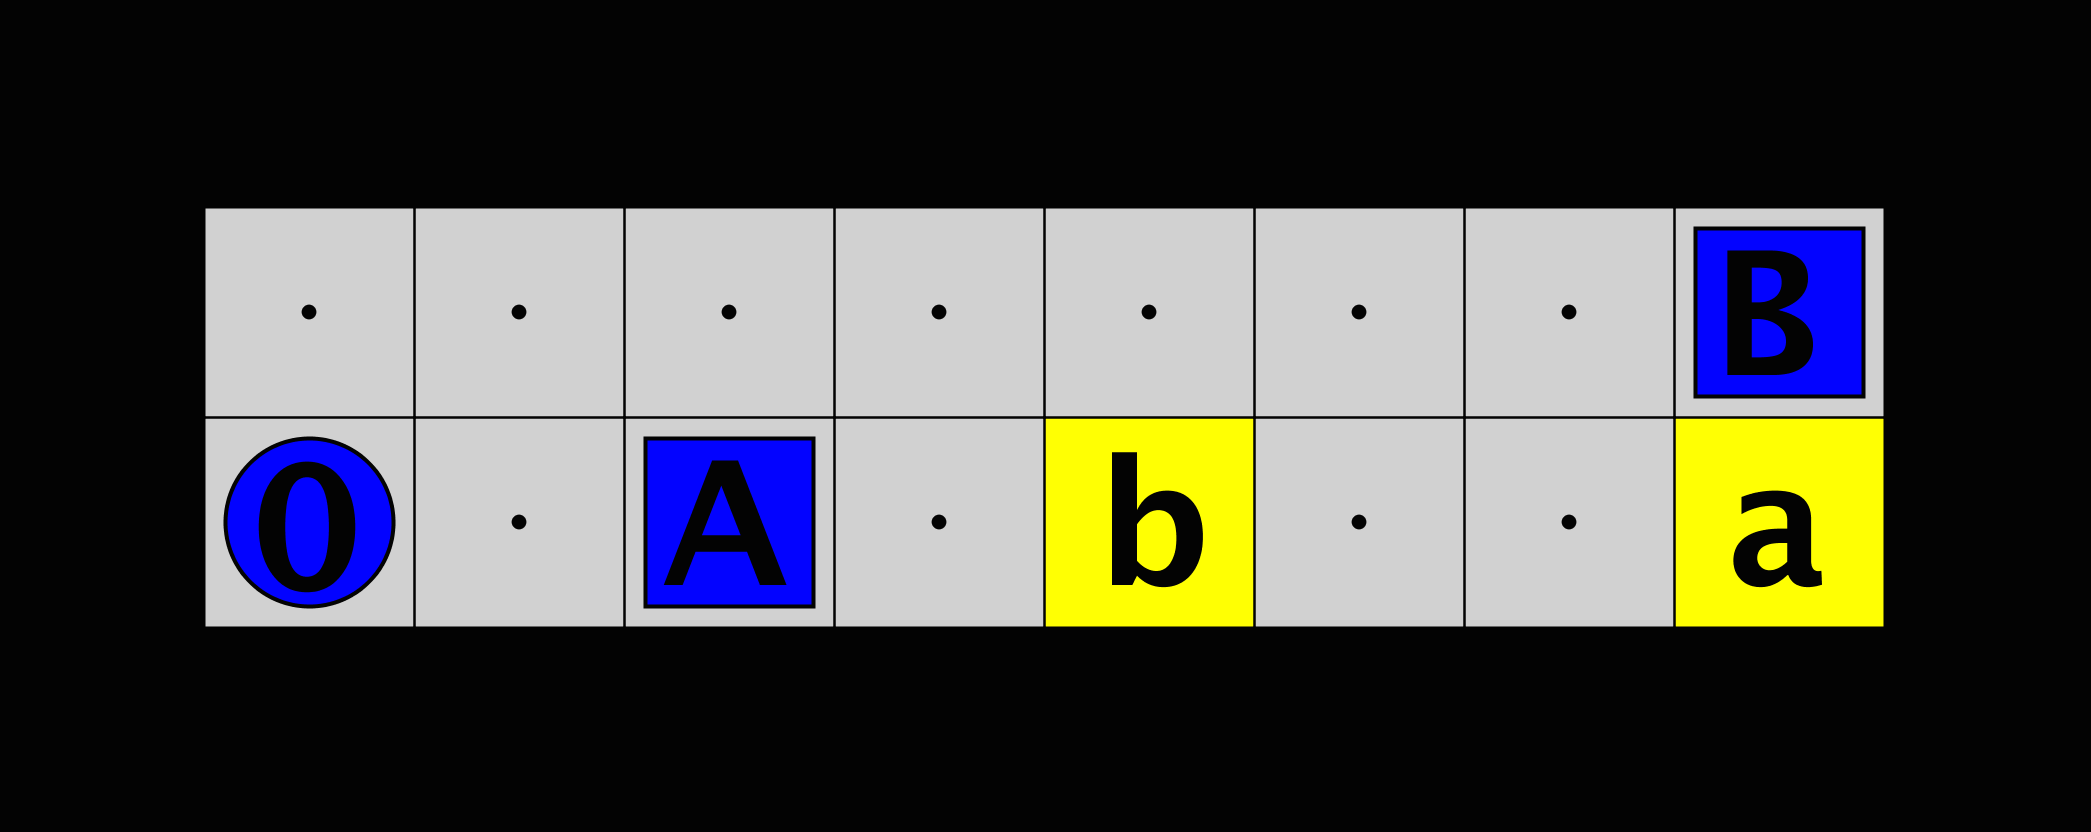
\includegraphics[width=0.3\textwidth]{conflict.png}
    \caption{Case that can be seen as a conflict, but can be avoided}
    \label{fig:conflict_avoidable}
\end{figure}


In this case, the solution to the relaxed problem, will involve the agent pushing box ``A'' through the goal ``b''. This is however not a real conflict, as the agent could just move the box around the goal ``b'', should it already be solved at the time it is solving ``a''. A simple way of trying to avoid this, is to do a check on the cells surrounding the goal. 
The conflict found in the case above will be determined as being avoidable, and hereby not trigger any ordering constraint between goal ``a'' and ``b''. 


\textit{Size prioritizing} 

THe length of the solution to the relaxed problem is used for prioritizing goals. 

The relaxed problem is based on the initial state of the level, hence the solution size to the relaxed problem will only somewhat apply to the first solved goal, as the agent's location will not be that of the initial state when solving the next goal. 



% Goal decomposition
\subsubsection{Goal decomposition}
In an effort to make the search algorithm as simple as possible, it is desired to divide the goals into clearly identified individual subgoals. A situation it is an advantage to decompose a goal in our client's domain, could be the situation where a box is blocking the path for an agent moving another box towards a goal. In order to avoid creating complex and computational heavy heuristics taking all parts of a level into account, the goal decomposition allows us to only consider few elements at a time. The path used to find conflicting boxes, is the path found by solving the relaxed problem for each goal.

The goal is decomposed into subgoals where each subgoal consists of a box that is blocking the path, and a cell where the box should be moved to so that it no longer blocks the path. The subgoals are sorted in the order in which the appear to be blocking the path to the actual goal. The subgoals are assigned to the goal, such that the subgoals should be completed before the client considers solving the actual goal. This is done by creating a specific case for the heuristics when subgoals exists on a goal. The heuristics is described in \autoref{sec:method_heuristics}. 

The implication of this approach to goal decomposition, using the path that is found by solving the goals as relaxed problems in the initial state, is that some of the created subgoals might not pose a conflict anymore, as the level and agent locations are changed. It is a very naive implementation that believes that the, in the beginning determined path, is the correct path. 



% Full search algorithm
\subsubsection{Search algorithm}
Inspired by the POP algorithm each goal is solved one by one, without regarding the completion of the level, but simply considering the level solved when there are no more goals to solve. The implication of this is that the client will most likely not find the optimal solution, as an optimal solution for many levels requires the agent to move boxes along when traveling towards other boxes. A case like this can be seen in \autoref{fig:non_optimal}:
\begin{figure}[h!]
    \centering
    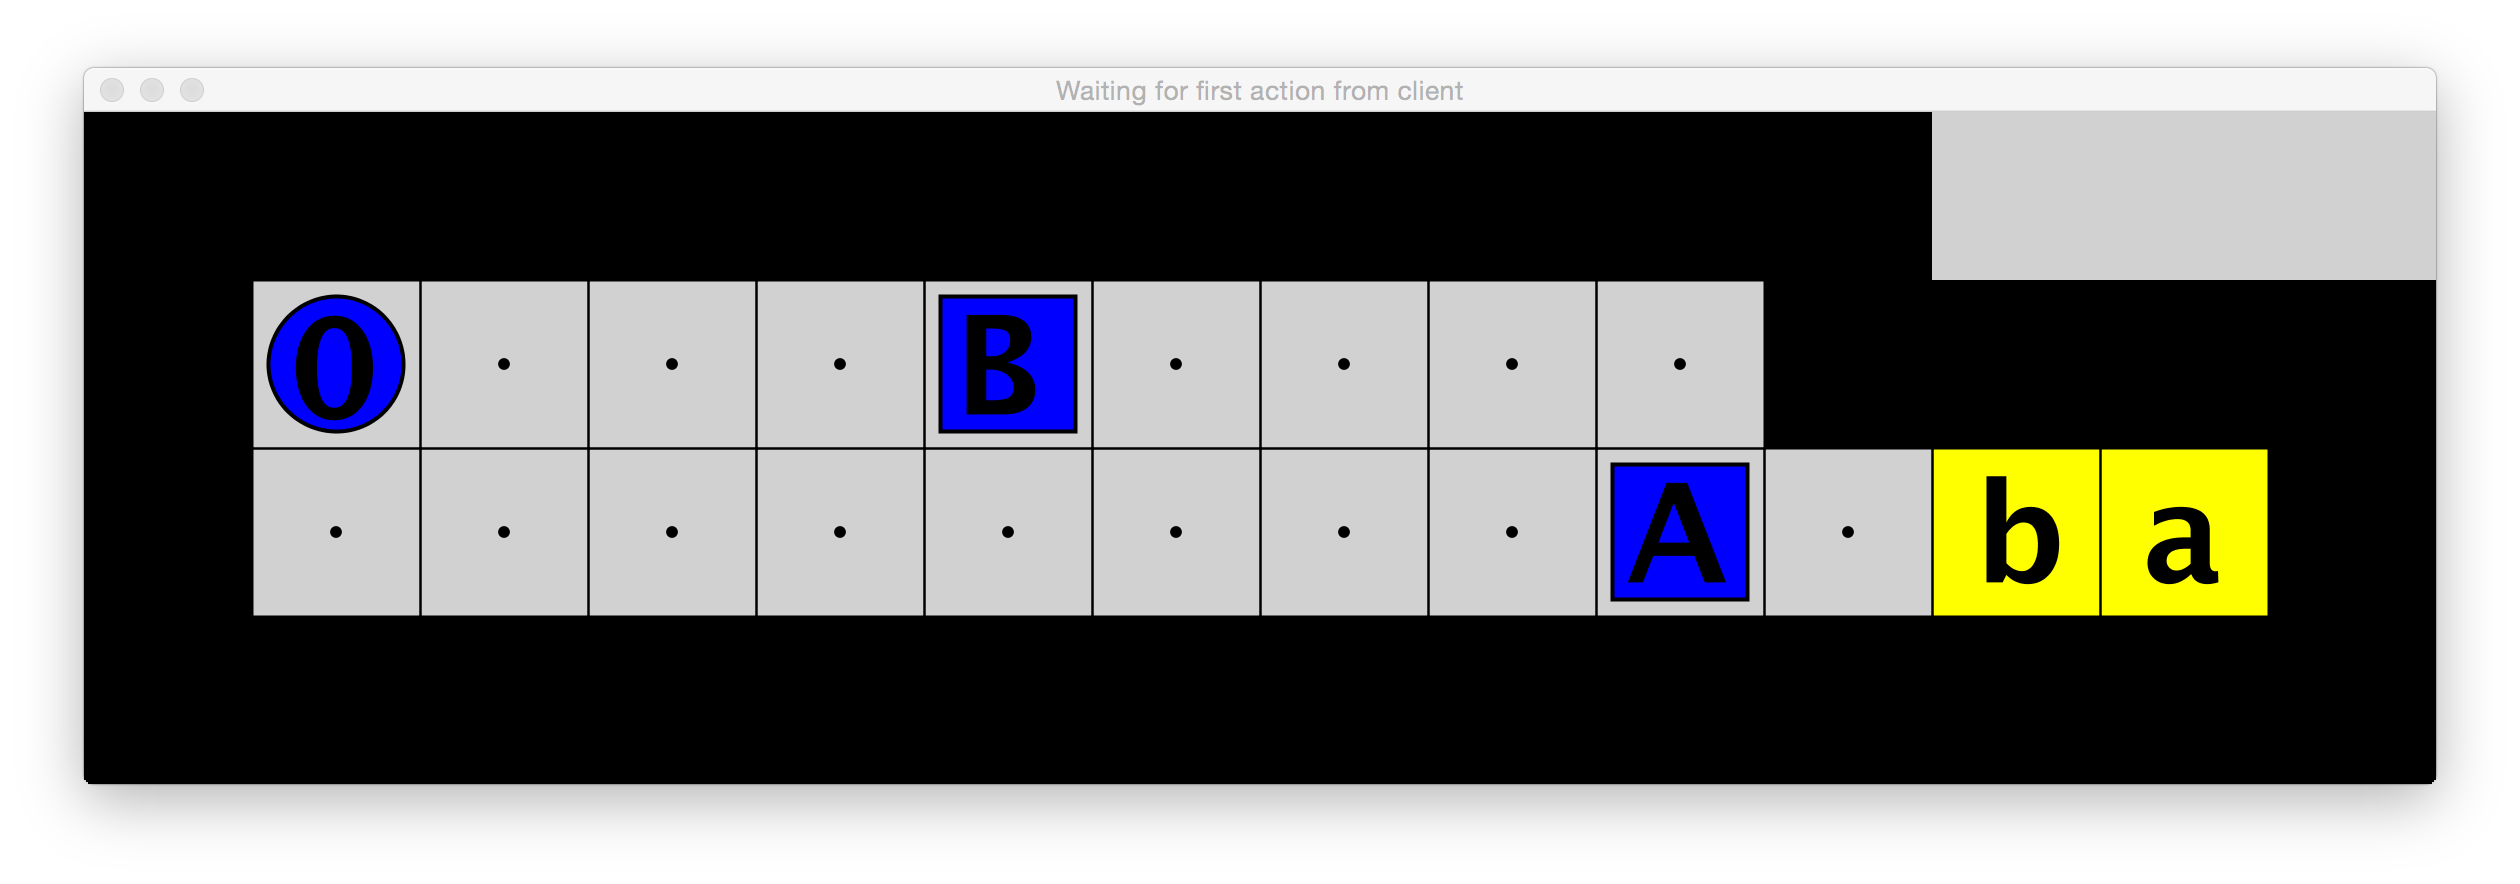
\includegraphics[width=0.3\textwidth]{non_optimal.png}
    \caption{Level with suboptimal solution.}
    \label{fig:non_optimal}
\end{figure}




% Backtracking algorithm
\subsubsection{Backtracking}

Inspired by partial order planning we have introduced a backtracking algorithm in our client. Even with the goals ordered with regards to conflicts, situations can occur where the agent places itself in a spot where it can get out of, without breaking a goal. A such situation occurs in the level visible in \autoref{fig:backtrack1}:
\begin{figure}[h!]
    \centering
    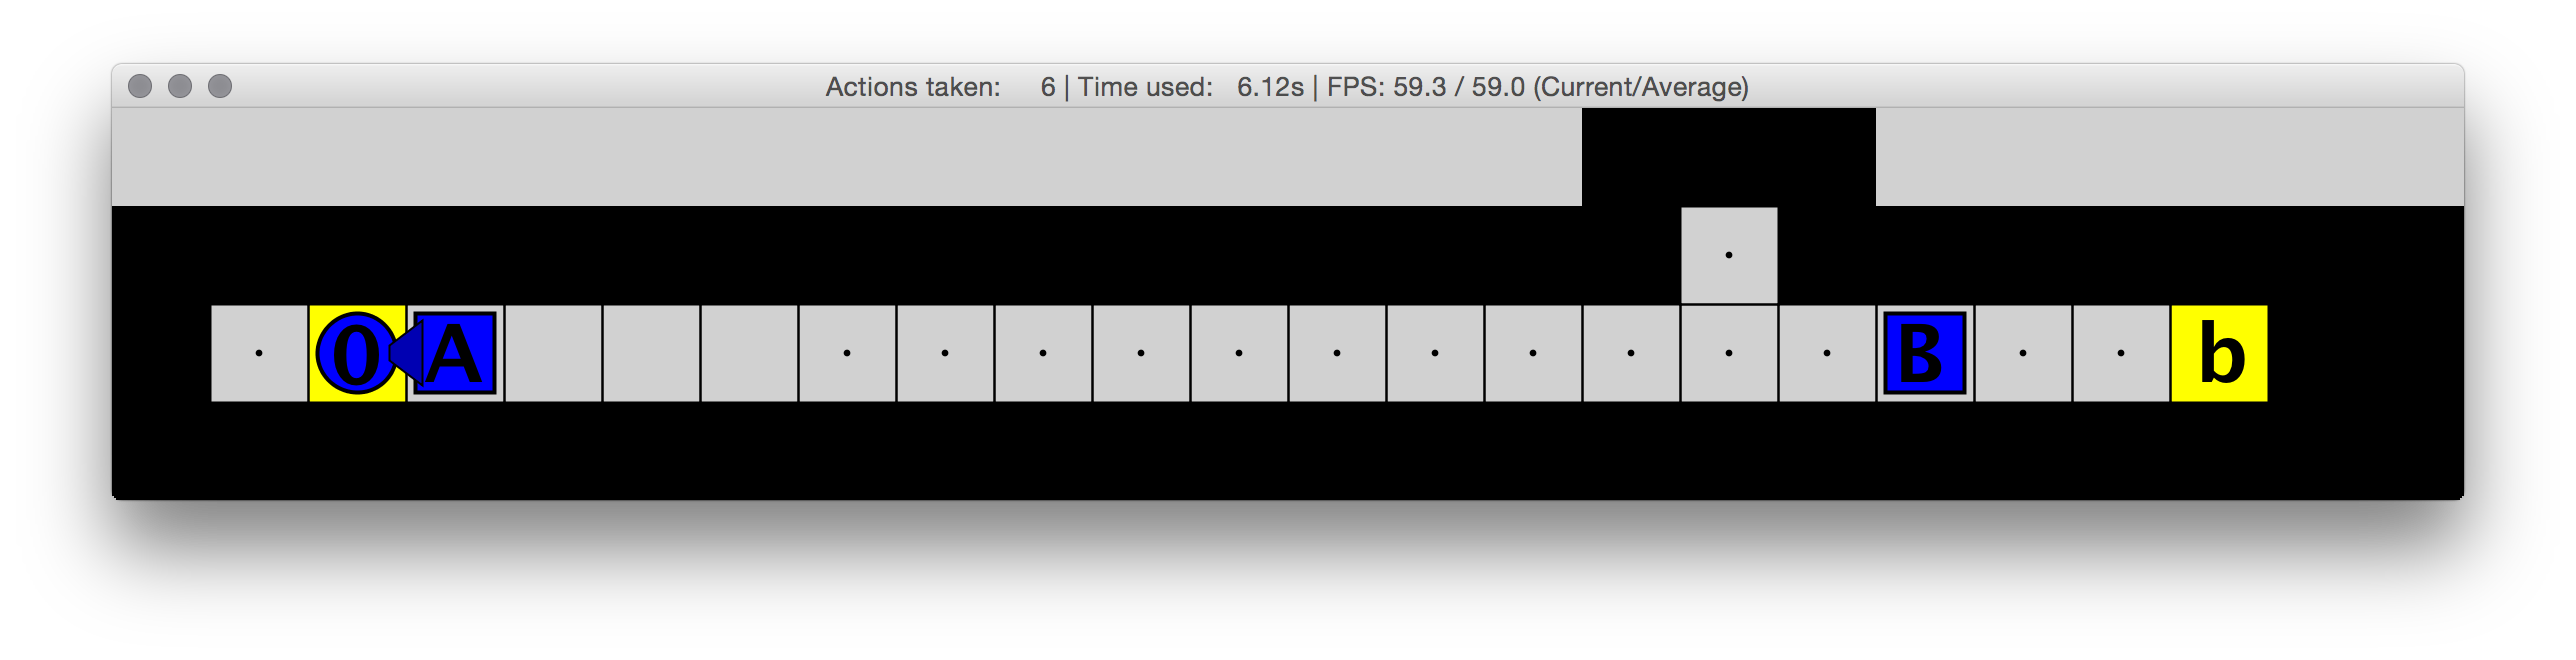
\includegraphics[width=0.5\textwidth]{backtrack1.png}
    \caption{Agent 0 on the way to place itself behind solved goal A.}
    \label{fig:backtrack1}
\end{figure}

When the agent solves a goal, it will proceed to solve the next goal assigned to it. In the above situation, any steps towards solving the next goal, will break the first. We regard this as unwanted behavior and do not allow it. Hence the agent doesn't have any possible moves and can't solve the goal. This is where backtracking comes into play. The agent's actions are backtracked to the immediate state before solving the last goal and the state representing the previously performed action to solve the goal is no longer reachable from that given state. From here, the agent will find an alternative solution to the goal. Once a solution is found, it will proceed to the next goal, the one it was actually trying to solve before backtracking. In the above example it produces the following action:
\begin{figure}[h!]
    \centering
    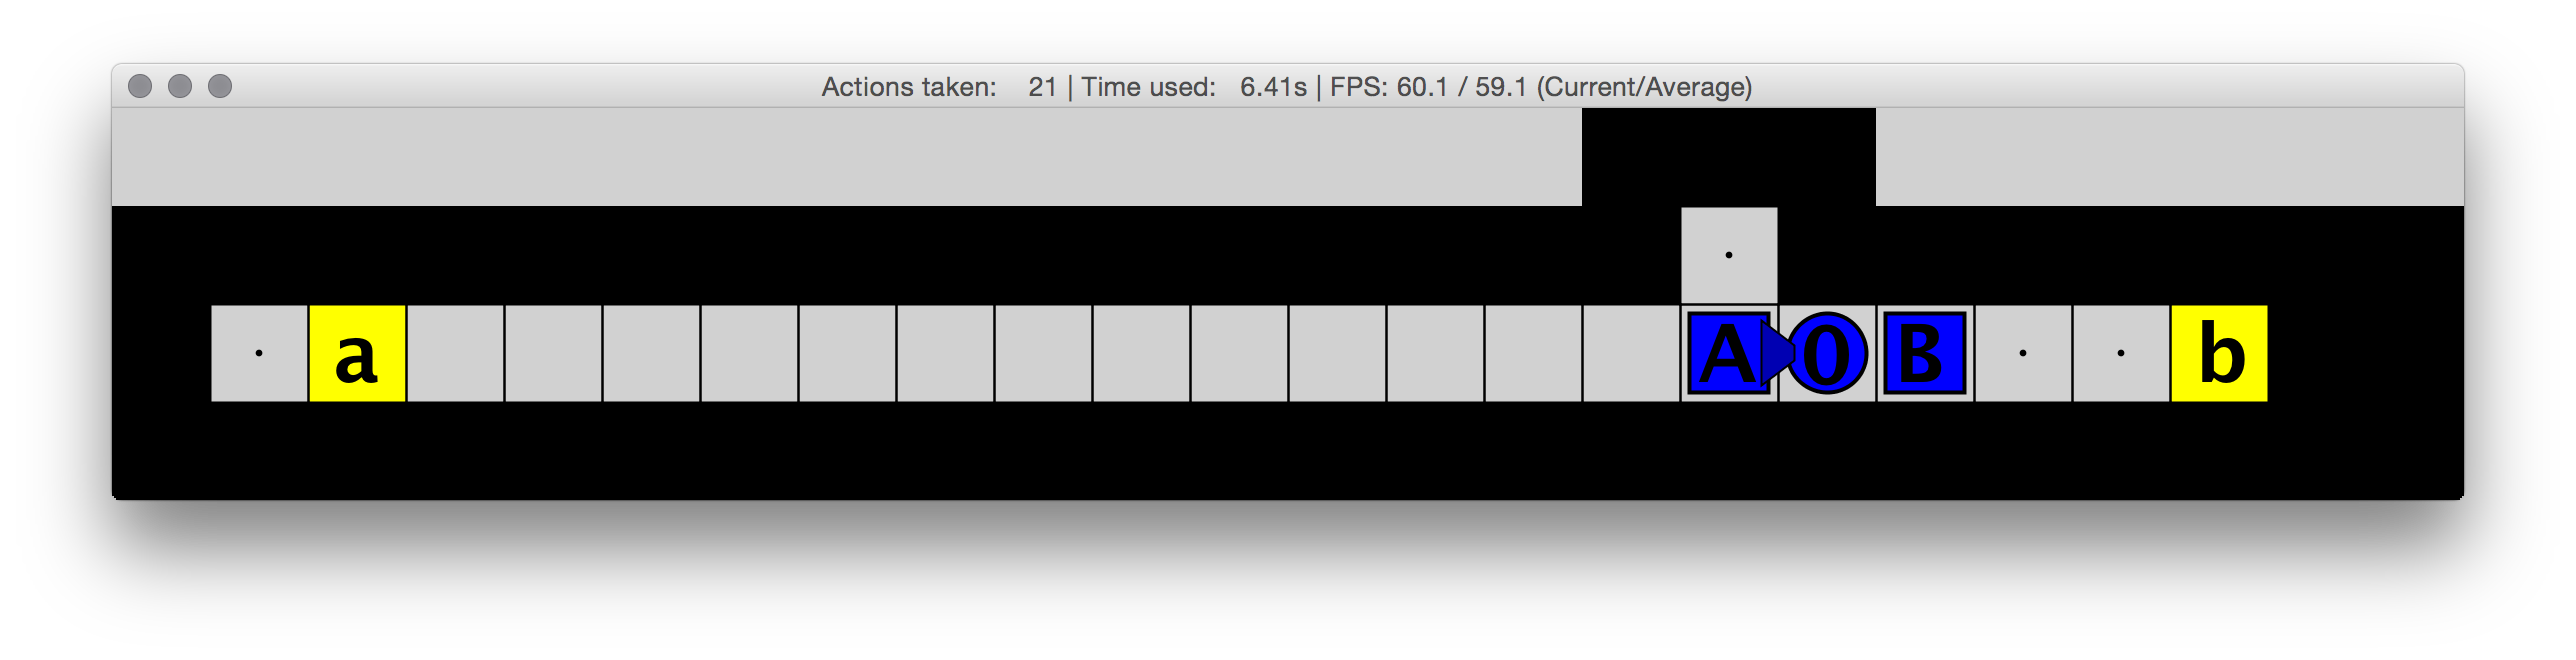
\includegraphics[width=0.5\textwidth]{backtrack2.png}
    \caption{Agent 0 finds alternative solution to goal A.}
    \label{fig:backtrack2}
\end{figure}






\subsection{POP - rename or move this ``??????????????????????'' }
% Partial order planning can be said to occur twice in the planning procedure, as the

Our planning procedure is somewhat inspired by partial order planning, as our client regards the individual goals as isolated as possible. 

The procedure consists of two major parts. The first part is a sort of ``all goals shortest path'' calculation as well as a determination of goal ordering / prioritizing. 
It is done as a relaxed problem search where the only components regarded are the goal to be solved, a box to solve it with, the agent to move the box, and the walls of the level. The relaxed problem is solved utilizing A\^{*} search strategy. 

The second part of our planning procedure  




% Heuristics
\subsubsection{Heuristics}
\label{sec:method_heuristics}
The heuristics implemented in the client is basically the distances between agent, boxes and goals. All distances used for heuristics are calculated as the Manhattan distance.  As the client is implemented to focus on solving a single goal, or subgoal, at a time, the heuristics can be simplified to favor actions that is helpful to solving that goal, whereas all other actions can be regarded as non-helpful. 
When regarding actions that involve the agent moving without a box, the distance calculated will be that between the agent, and the box it is supposed to solve a goal with. 

Actions where the agent either pushes or pulls a box, two situations exists; 1) moving the box suggested for solving a goal, or 2) moving a completely irrelevant box. 

In the first situation the heuristics will be the calculated distance between the box and the goal.

In the other situation the heuristics will be based on the distance between agent and the box it is supposed to solve the goal with, and the distance between that box and the goal. In order to discourage this action the distance is multiplied by a discouraging factor.


\textbf{Relaxed problem heuristics}

When doing relaxed problem search, the heuristics are based on the distance between the agent and the box, and the distance between the box and the goal. As those, include the walls, are the only elements in the level, there are no other complications to take into account. 



\textbf{Admissibility of heuristics}

As the heuristics are calculated as the Manhattan distance between agent and box, and box and goal, it is admissible. However, when non-helpful actions are considered, it is no longer the case due to the use of a discouraging factor. 
\todo[inline]{Bjarke!? Is this above paragraph correct?}


- Relaxed problem --> Only one goal, box and agents

- Picking a specific box for a goal
- Relies heavily on the goal order being correct and chosen boxes being correct



\subsection{Multi-agent} 

\todo[inline]{ FIX REFERENCE BJARKE !!!!! }

The implementation of the multi-agent client is somewhat inspired by the Generalized Partial Global Planning from \cite{Decker, K., Li, J}. 

The goals are ordered with regards to whether or not they disrupt or conflict with other subgoal plans \autoref{sect:subgoal_pop}. As the planning is executed sequentially in the determined goal order, and not concurrently, the communication between agents is simplified as the hierarchy of agents and plans is already established by the goal order. 
If an agent moves a box or occupies a cell at a given time, it is the other agents responsibility to comply with this and either wait or do something else. However, this practice relies on that the determined goal order is correct possible to complete. 

The communication is simply done by letting the agents announce which cells they occupy at a given time in the plan as well as which box they move, if any. The other agents' planning procedures are then affected by the occupied cells, such that the agents' are imposed a resource constraint, keeping them from trying to use resources that are busy. 

The communication of results between agents are done through the same announcing channels as mentioned above. As the execution is sequential, no actual notifications are sent, the information about results are just made available for all other agents to retrieve. Hard relationships are handled this way, such that if goal ``a'' must come before ``b'', the agent responsible for solving ``b'' cannot do this until ``a'' is solved.  


\todo[inline]{MORE MULTI AGENT STUFF !!!!!! }



\subsection{Shortcomings}
The developed multi-agent system implements a lot of clever ideas, but as in most cases concerning planners, all algorithms might have negative and non-foreseen implications in some special cases. This applies to our planner as well. 


\textbf{Bidding}

The bidding and choosing of boxes for solving goals has one dire weakness, that without re-planning, will leave the client unable to solve some levels. As the heuristics used for bidding favors boxes that are close to the goals, a situation can arise, where a box found to solve the relaxed problem, can't be used to solve the actual problem. A such situation arises in the level illustrated in \autoref{fig:shortcomings_bid}. As a goal is attempted to solve with the nearest box, the goal ordered to be solved first, will be attempted to be solved with the box furthest away from it, as all other boxes are taken. In the relaxed problem, this poses no issue and is easily solved. In the full problem, the boxes cannot be re-arranged, such that the chosen box can be used to solve the goal. THe client could however benefit from just taking any other box to solve to goal with. 
\begin{figure}[h!]
    \centering
    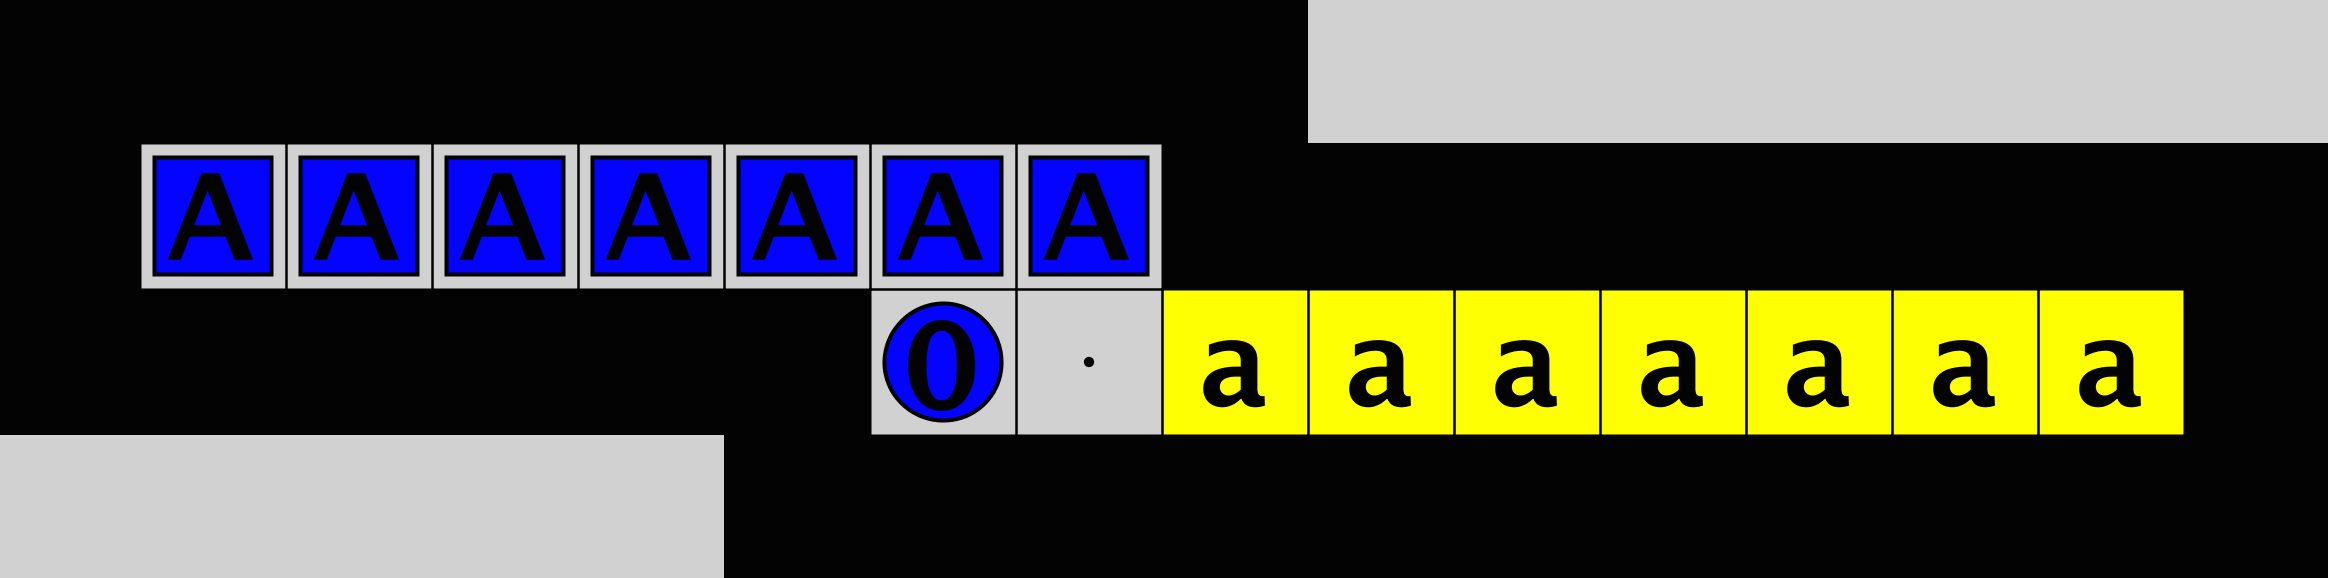
\includegraphics[width=0.3\textwidth]{shortcomings.png}
    \caption{A level where the bidding and choosing of boxes to solve goals with can pose a problem.}
    \label{fig:shortcomings_bid}
\end{figure}



\textbf{Backtracking limitation}

There is currently no backtracking failsafe which means that the backtracking algorithm could possibly end up backtracking to the initial state and not find any allowed actions, resulting in the level not being solved. 
At this point the client should repeat the planning with another approach than the one recently explored. 



\textbf{Multi-agent and goal decomposition}

The multi-agent communication, along with the goal decomposition lacks a very important feature. The ability for agents to request help from other agents. In the case of the level seen in \autoref{fig:shortcomings_multi}, agent ``0'' will decompose goal ``a'' and create a subgoal that it cannot solve. Specifically the moving of box ``B'', which only agent ``1'' is capable of. 
\begin{figure}[h!]
    \centering
    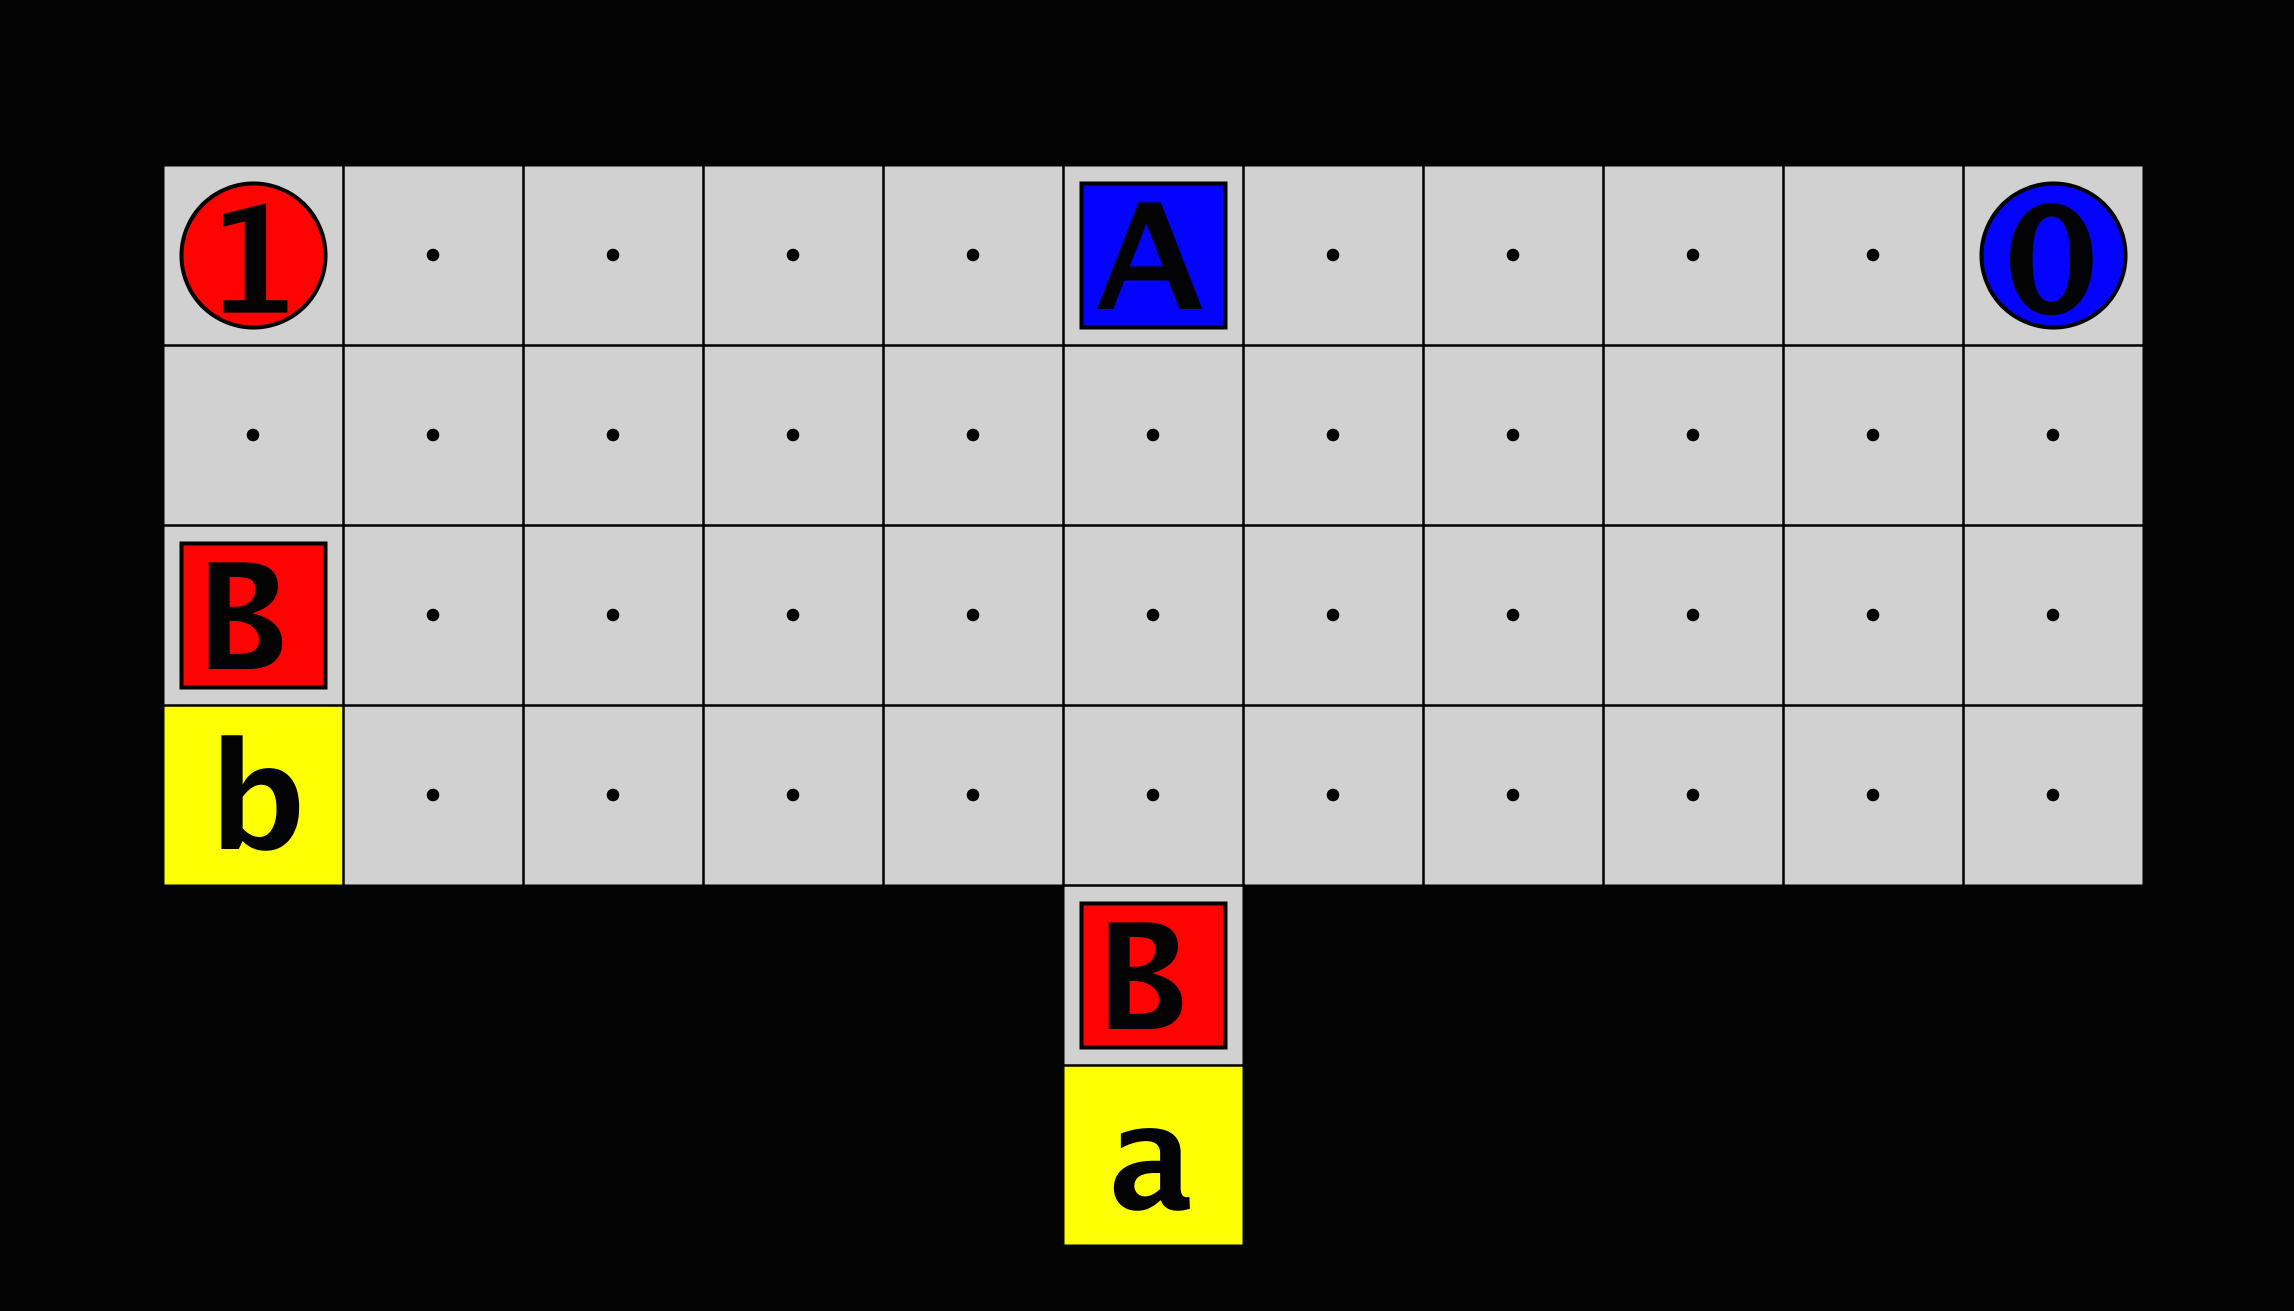
\includegraphics[width=0.3\textwidth]{shortcomings_multi.png}
    \caption{A level where communication and goal decomposition is inadequate.}
    \label{fig:shortcomings_multi}
\end{figure}


\textbf{In general} the developed client relies heavily on the determined goal order being correct. Should it not be, the client is left to chance. 

\end{document}
